
\chapter{Anforderungsanalyse}\label{chap:requirements-analysis}

    \section{Zielsystem und Kontextabgrenzung}\label{sec:target-system-and-context-delimitation}
        \subsection{Systemgrenzen und Anwendungsbereich}\label{subsec:system-boundaries-and-application-scope}
            Das System soll einen nichtplanaren 6 achsigen Slicer sowie eine dazugehörige Robotersteuerung abbilden.
            Hierfür wird ein 3D-Objekt im \ac{STL}-Format eingelesen.
            \ac{medusa} berechnet daraus die Pfade, die der Druckkopf zurücklegen soll.
            Aus diesen Pfaden generiert \ac{kronos} die Steuerung für den simulierten Roboterarm.
            Es wird nur in einer Simulation gearbeitet.
            Faktoren wie die Materialextrusion oder andere physischen Einflüsse werden vernachlässigt,
            \sig{Nik Wachsmann}

        \subsection{Stakeholder und Nutzungsszenarien}\label{subsec:stakeholders-and-usage-scenarios}
            Das System wird für Forschungszwecke entwickelt.
            Es soll so ausgelegt werden, dass Entwickler und Prüfer mithilfe einer Anleitung das Programm bedienen können.
            Für die weitergehende Entwicklung oder aufbauende Projekte sollen die Schnittstellen des Programmes eindeutig definiert sein.
            Es wird explizit nicht auf Benutzerfreundlichkeit für Endnutzer entwickelt.
            \sig{Nik Wachsmann}

        \subsection{Randbedingungen des Einsatzkontexts} \label{subsec:boundary-conditions-of-deployment-context}
            Aufgrund der experimentellen Natur des Projektes wird nicht explizit für Kompatibilität entwickelt.
            \ac{medusa} wird getrennt von \ac{kronos} entwickelt.
            \ac{kronos} wird in einer Docker Umgebung entwickelt, um die Schnittstelle zu \ac{ROS}~2, MoveIt und RViz einheitlich zu halten.
            Die Programme werden für typische Hardware und ohne Echtzeitanforderungen entwickelt.
            Ein moderner Computer soll in der Lage sein, die Programme auszuführen.
            \sig{Nik Wachsmann}
  

    \section{Methodik der Anforderungserhebung}\label{sec:requirements-elicitation-methodology}
        \subsection{Informationsquellen und Datengrundlage}\label{subsec:information-sources-and-data-basis}
            Die Anforderungen an das System wurden primär aus dem fachlichen Kontext des 6-achsigen 3D-Drucks sowie aus verwandten wissenschaftlichen Arbeiten zu nichtplanaren Slicing-Verfahren und mehrachsiger Roboterkinematik abgeleitet.
            Ergänzend dienten die Dokumentation der verwendeten Softwareframeworks \ac{ROS}~2, MoveIt und RViz als technische Informationsquellen, da diese die implementierbaren Steuerungsstrategien direkt einschränken.
            Zur Abgrenzung des Systemumfangs wurden außerdem die Limitationen konventioneller kartesischer 3D-Drucker und bestehender Slicing-Werkzeuge analysiert.
            Die identifizierten Anforderungen wurden nicht durch formale Nutzerbefragungen erhoben, da das System ausschließlich für Forschungs- und Entwicklungszwecke vorgesehen ist
            und keine definierten Endnutzer besitzt.
            \sig{Nik Wachsmann}

        \subsection{Vorgehen zur Konsolidierung von Anforderungen} \label{subsec:approach-for-consolidating-requirements}
            Aufgrund der Aufteilung in die Module \ac{medusa} und \ac{kronos} wurden die Anforderungen schrittweise in einem iterativen Prozess zusammengeführt.
            Dabei wurde stetig geprüft, ob die von \ac{medusa} generierten geometrischen Daten (Punkte und Normalen)
            für die kinematischen Solver von \ac{kronos} (MoveIt) ausreichend und verwertbar sind.
            Unstimmigkeiten bei der Datenaustausch-Schnittstelle wurden in Abschnitt \ref{subsubsec:requirements-software-interfaces} aufgelöst,
            um eine lose Kopplung und damit eine unabhängige Entwicklung der Teilsysteme zu gewährleisten.
            \sig{Nik Wachsmann}

        \subsection{Priorisierung und Bewertungslogik}\label{subsec:prioritization-and-evaluation-logic}
            Die Priorisierung erfolgt nach dem \ac{MOSCOW}-Schema, um den experimentellen Charakter des Projekts zu berücksichtigen:
            \paragraph{Must-Have:}
            Korrekte Pfadberechnung nichtplanarer Schichten,
            Einlesen von \ac{STL}-Daten,
            kollisionsfreie Simulation der Armbewegung,
            Visualisierung der Trajektorien in einer 3D-Ansicht.
            \paragraph{Should-Have:} Handhabung extremer Überhänge (90°).
            \paragraph{Could-Have:} Unterstützung zusätzlicher Dateiformate, grafische Benutzeroberfläche zur Parametrierung.
            \paragraph{Won't-Have:} Physische Extrusion, Echtzeit-Ansteuerung realer Hardware, automatische Fehlerkorrektur bei defekten \ac{STL}-Netzen.
            \sig{Nik Wachsmann}

    \section{Funktionale Anforderungen}\label{sec:functional-requirements}
        \subsection{Anforderungen an Medusa}\label{subsec:medusa-requirements}

            \paragraph{Anforderungen}
            Das Teilsystem \ac{medusa} des Zielsystems soll aus einfachen 3D-Objekten, die gewisse Einschränkungen einhalten,
            Toolpaths für ein 6-achsiges 3D-Druck System berechnen können.
            Für die Pfadplanung kann die Schichtdicke festgelegt werden.
            Zusätzlich soll \ac{medusa} für nichtplanare Slicing-Verfahren adaptive Layerhöhen unterstützen,
            sodass die Schichtdicke entlang eines Pfades oder zwischen benachbarten Pfaden abhängig von lokaler Geometrie,
            Krümmung und Überhangsituation variiert werden kann.
            Diese Schichtdicken werden für den Bahnabstand und den Vorschub verwendet, nicht für die Materialextrusion. 
            Die Berechnung beschränkt sich rein auf die Bahnplanung des Extruders mit Position und Drucknormalen für jeden Punkt.
            Hierbei ist das Ziel, nichtplanare Pfade zu erzeugen.
            Nichtplanare Pfade bezeichnen Pfade, deren Trajektorien nicht vollständig innerhalb einer Ebene parallel zur Druckplatte verlaufen.
            Dabei können einzelne Schichten weiterhin planar sein, sofern sie in einem Winkel ungleich $0^\circ$ zur Druckplatte liegen.
            
            \paragraph{Ein- und Ausgabe}
            Das Programm akzeptiert 3D Modelle mindestens im \ac{STL}-Format.
            Weitere Formate können, müssen aber nicht akzeptiert werden.
            Eingabemodelle müssen geschlossene, manifoldfähige Dreiecksnetze ohne Selbstüberschneidungen darstellen.
            Die Geometrie der 3D-Objekte darf keine horizontalen Kavitäten, internen Hohlräume oder Brückenstrukturen, 
            die eine Vereinigung von zwei getrennten Pfaden in der Horizontalen erfordern enthalten.
            Ausgeschlossen hiervon sind Überhänge, die in freier Luft beginnen.
            \ac{medusa} liefert als Ausgabe eine geordnete Liste an Pfadpunkten, die aus Position im Objektkoordinatensystem sowie deren Drucknormale bestehen.

            \paragraph{Out of Scope}
            Bei der Pfadplanung werden keine Füllmuster verwendet.
            Die Objekte werden als Massiv angenommen und mit einem 100\%-Infill (Solid) geplant.
            Bei Überhängen wird die Druckrichtung angepasst und es werden keine Stützkonstruktionen hinzugefügt.
            Die benötigte Materialextrusion, die für den physischen Druck benötigt wird, wird nicht mit berechnet.
            \sig{Nik Wachsmann}
        
        \subsection{Anforderungen an KRONOS}\label{subsec:kronos-requirements}

            \paragraph{Anforderungen}
            Das Teilsystem \ac{kronos} des Zielsystems soll die generierten Pfade aus \ac{medusa} einlesen und diese in Roboterarm-Bewegungen überführen.
            Hierbei soll die Bewegung zwischen zwei Punkten des Pfades linear im kartesischen Raum ablaufen.
            Diese Pfadpunkte bestehen aus einer Position und einer Drucknormalen im Objektkoordinatensystem.
            Für die Bewegungsplanung werden die Pfadpunkte vom Objektkoordinatensystem in das globale Koordinatensystem transformiert,
            um es auf der virtuellen Druckplatte zu Plazieren.
            Bei der Bewegungsplanung werden nur die physischen Limits des Roboterarms für die Pfadplanung beachtet,
            sodass keine Gelenkgrenzen oder offensichtlichen Singularitäten verletzt werden.
            Pfade, die Singularitäten enthalten, werden als nicht ausführbar markiert

            \paragraph{Ein- und Ausgabe}
            Die Eingabe für \ac{kronos} ist die geordnete Liste an Pfadpunkten, die \ac{medusa} berechnet.
            Da \ac{medusa} diese Limits des Roboters nicht kennt, können Pfade entstehen, die der Roboter nicht nachfahren kann.
            Die Ausgabe von \ac{kronos} ist die Steuerung des Roboterarms mithilfe von \ac{ROS}~2 und MoveIt.

            \paragraph{Out of Scope}
            Bei der Bewegungsplanung wird die Kollisionserkennung zwischen dem Roboter und dem theoretisch bereits gedruckten Teil des 3D Objektes vernachlässigt.
            Ebenso wird die Extrudergeometrie sowohl bei der Bewegung sowie der Kollisionsberechnung ignoriert.
            So wie \ac{medusa} wird auch bei der Roboteransteuerung die Materialextrusion nicht berücksichtigt.
            Da die Materialextrusion nicht beachtet wird, wird auch die Bewegungsgeschwindigkeit nicht konstant gehalten.
            \sig{Nik Wachsmann}
        
        \subsection{Anforderungen an Hardware}
            \paragraph{Anforderungen}
            Die Ansteuerung tatsächlicher Hardware ist nicht Teil des Zielsystems.
            Die Hardware wird mit \ac{ROS}~2 und RViz simuliert.
            Diese Simulationsumgebung erlaubt das nahtlose Einbinden eines physischen Roboterarms wenn dies gewünscht ist.
            Diese Entscheidung wurde getroffen, um nicht durch Softwarefehler die Hardware zu beschädigen.

            \paragraph{Out of Scope}
            Es wird keine spezialisierte Hardware für das System entwickelt.
            Es wird keine Hardware vorbereitet, um das Drucken zu erlauben.
            \sig{Nik Wachsmann}

        
        \subsection{Testmodelle}\label{sec:testmodels}
            Für das Testen der slicing-Algorithmen werden vier inkrementell komplexere 3D Objekte verwendet.

            \paragraph{Würfel}
            Der Würfel dient als Referenzobjekt.
            Es gibt keinen Überhang und alle Schichten haben die gleiche Größe.

            \paragraph{Doppelte Pyramide}
            Die doppelte Pyramide wird für das Verhalten bei der Verkleinerung von Druckschichten sowie leichten Überhängen verwendet.
            
            \paragraph{Einfaches T}
            Das einfache T wird für starke Überhänge von 90° gewählt.
            Beim normalen Drucken würde es auf dem Kopf gedruckt werden, um Stützen zu vermeiden, doch hier wird es als Test verwendet.

            \begin{figure}[htb]
                \centering
                % Sobald du das Bild hast: \includegraphics[width=\textwidth]{testmodelle.png}
                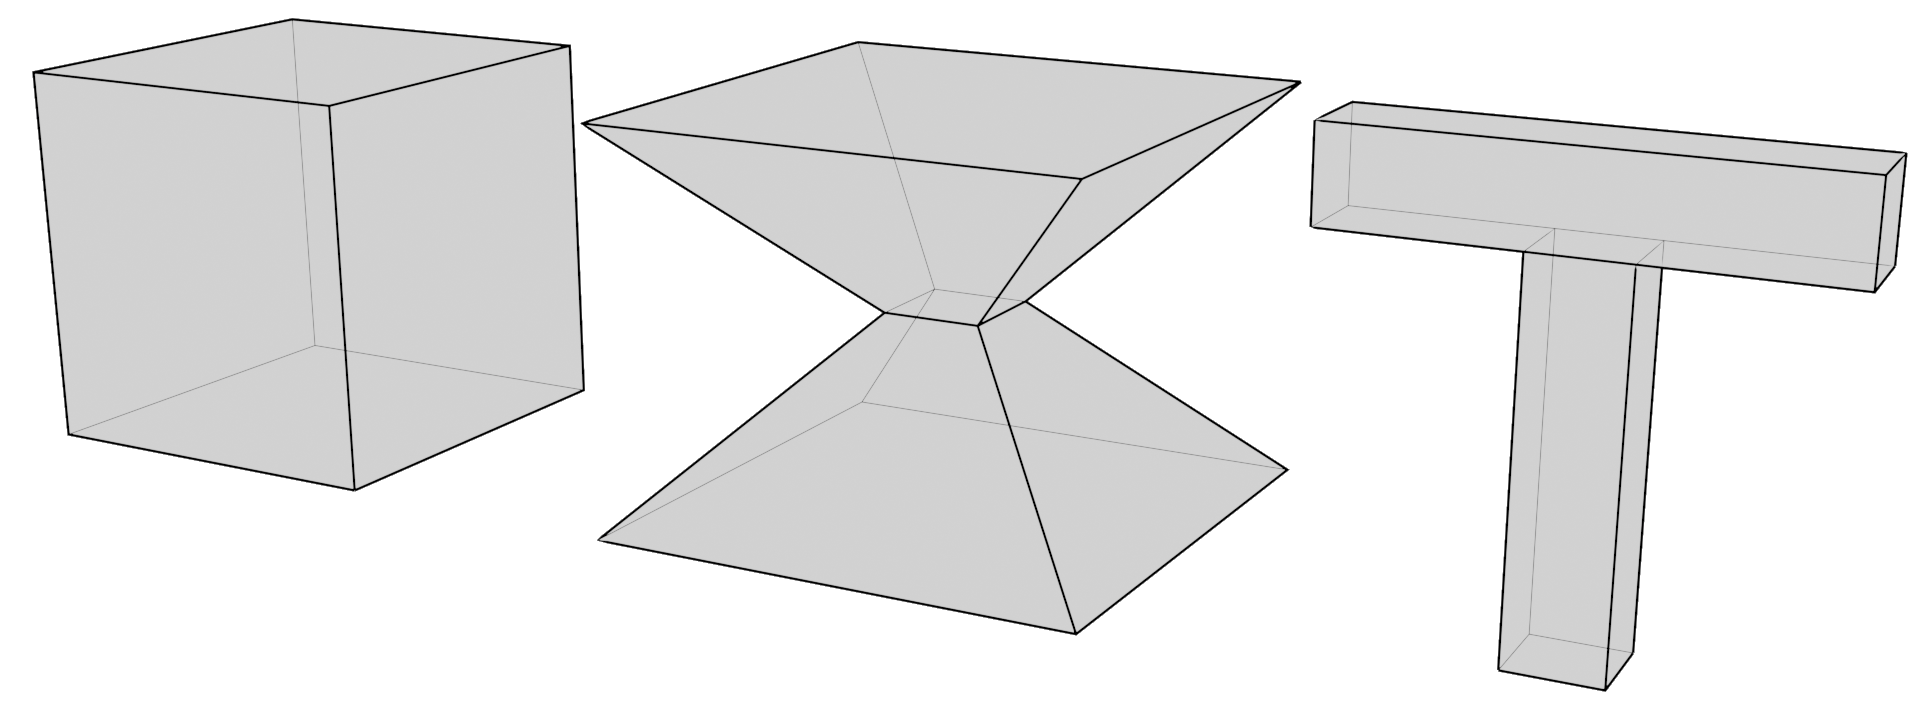
\includegraphics[width=0.8\textwidth]{dependencies/pictures/example_objects.png}
                \caption{Die drei Testmodelle: Würfel, Doppelte Pyramide und Einfaches T.}
                \label{fig:testmodels}
            \end{figure}

            Diese Modelle decken die wesentlichen geometrischen Herausforderungen des 6-achsigen Druckens ab,
            von der einfachen Schichtzustellung bis hin zur Ausrichtung der Drucknormale bei komplexen Überhängen.
            Sie beinhalten nur Objekte, die nach den \ac{medusa} Systemgrenzen erlaubt sind.
            \sig{Nik Wachsmann}

    \section{Nicht-funktionale Anforderungen}\label{sec:non-functional-requirements}
        \subsection{Leistungs-, Genauigkeits- und Robustheitsanforderungen}\label{subsec:performance-accuracy-and-robustness-requirements}
            Die Berechnungszeit für die definierten Testmodelle darf auf einer gängigen Entwickler Workstation einen Zeitrahmen von wenigen Minuten nicht überschreiten,
            um iterative Testzyklen zu ermöglichen.
            Das Programm muss nicht für den Normalverbraucher optimiert sein.
            Größere oder komplexere Modelle werden nicht beachtet.
            Die Abweichung der generierten Bahnen von der Originalgeometrie muss innerhalb der durch die Schichtdicke und den Düsendurchmesser definierten Toleranzen liegen.
            Bei fehlerhaften Eingaben wird das Programm abgebrochen.
            Die erzeugten Ergebnisse müssen reproduzierbar sein.
            \sig{Nik Wachsmann}

        \subsection{Anforderungen an Wartbarkeit und Erweiterbarkeit}\label{subsec:requirements-for-maintainability-and-extensibility}
            Die Software soll modular aufgebaut werden, um Anpassungen und Erweiterungen zu erleichtern.
            Hierbei wird das Projekt in \ac{medusa} und \ac{kronos} unterteilt.
            Diese beiden Komponenten werden separat in logische Module geteilt.
            Alle Schnittstellen müssen eindeutig definiert und dokumentiert sein.
            Hierbei sind die Eingaben zu \ac{medusa}, die Daten von \ac{medusa} nach \ac{kronos} und die Ausgabe von \ac{kronos} zu definieren.
            Insbesondere sollen neue Slicingalgorithmen einfach hinzuzufügen sein.
            \sig{Nik Wachsmann}

        \subsection{Anforderungen an Sicherheit und Zuverlässigkeit}\label{subsec:requirements-for-safety-and-reliability}
            Um die Sicherheit der Hardware zu gewährleisten werden die generierte Pfade nur in der Simulation getestet.
            Hierbei müssen Gelenkgrenzen und Singularitäten, insbesondere jedoch Kollisionen des Roboterarms mit sich selbst beachtet werden.
            Da dies kein Produktivsystem ist werden Fehler nicht automatisch vom Code behoben.
            Bei fehlerhaften Eingaben oder Berechnungen wird das Programm abgebrochen, sodass der Anwender den Fehler beheben kann.
            \sig{Nik Wachsmann}
        
        \subsection{Anforderungen an die Benutzbarkeit}\label{subsec:requirements-for-usability}
            Da dies ein experimentelles System ist muss die Oberfläche nicht für Endnutzer entwickelt werden.
            Das System soll für Entwickler mit geringem Einarbeitungsaufwand und einer begleitenden Dokumentation bedienbar sein.
            Für die Darstellung des berechneten Pfades wird eine 3D-Ansicht benötigt.
            Weitere Eingaben können über eine \ac{GUI} erfolgen, jedoch ist eine Kommandozeile ausreichend.
            Die simulierte Bewegung des Roboterarms muss in einer 3D Ansicht erfolgen.
            \sig{Nik Wachsmann}

    \section{Schnittstellen- und Integrationsanforderungen}\label{sec:interface-and-integration-requirements}
        \subsubsection{Softwareseitige Schnittstellen}\label{subsubsec:requirements-software-interfaces}
            Die Kommunikation zwischen \ac{medusa} und \ac{kronos} erfolgt über genau ein gemeinsames Datenartefakt,
            das den vollständigen Fertigungsauftrag beschreibt.
            Dieses Artefakt muss alle für die Ausführung notwendigen Informationen enthalten,
            sodass \ac{kronos} den Auftrag ohne Zugriff auf interne Datenstrukturen oder Zwischenergebnisse von \ac{medusa} verarbeiten kann.
            Die Schnittstelle ist persistent und asynchron:
            zwischen Erzeugung und Ausführung können beliebig lange Zeiträume liegen, und beide Komponenten müssen nicht gleichzeitig oder auf derselben Maschine laufen.
            Der Austausch soll sowohl automatisiert, etwa als Teil einer Werkzeugkette, als auch manuell durch den Nutzer erfolgen können.
            Die Schnittstelle wird bewusst einfach und schwach gekoppelt gehalten, damit beide Komponenten unabhängig voneinander weiterentwickelt,
            getestet und bei Bedarf durch andere Komponenten ersetzt werden können, solange das vereinbarte Übergabeformat eingehalten wird.
            \sig{Nik Wachsmann}

        \subsection{Hardware- und Steuerungsschnittstellen} \label{subsec:hardware-and-control-interfaces}
            Die Ansteuerung des Roboters erfolgt in \ac{kronos} über \ac{ROS}~2 in Verbindung mit MoveIt.
            \ac{medusa} selbst kommuniziert nicht direkt mit dem Roboter, sondern liefert ausschließlich die zu verfahrenden Pfade.
            \ac{kronos} übernimmt darauf aufbauend die Bahnplanung und Bewegungssteuerung des Roboterarms.
            Durch die Nutzung einer \ac{ROS}~2-basierten Steuerungsarchitektur kann zwischen simulierter und physischer Hardware unterschieden werden,
            ohne dass Änderungen an der Pfadverarbeitung in \ac{kronos} erforderlich sind.
            Damit ist die Software grundsätzlich so aufgebaut,
            dass der Übergang von einer simulierten Ausführungsumgebung auf ein reales Robotersystem mit möglichst geringem Anpassungsaufwand erfolgen kann.
            Die Ansteuerung eines Extruders oder eines weiteren Prozesswerkzeugs ist im Rahmen dieses Projekts nicht vorgesehen.
            Der Fokus liegt ausschließlich auf der Bahnplanung und Bewegungsausführung des Roboterarms.
            \sig{Nik Wachsmann}

        \subsection{Datenformate und Austauschprotokolle}\label{subsec:data-formats-and-exchange-protocols}
            Als Eingabeformat für die zu verarbeitenden 3D-Modelle wird \ac{STL} verwendet.
            Weitere Formate sind prinzipiell denkbar, werden im Rahmen dieses Projekts jedoch nicht betrachtet.
            Der Datenaustausch zwischen \ac{medusa} und \ac{kronos} wird in Abschnitt \ref{subsubsec:requirements-software-interfaces} definiert.
            Ein komplexes Netzwerkprotokoll ist für den aktuellen Projektumfang nicht erforderlich, da die Kopplung der beiden Systeme über den Dateiaustausch erfolgt.
            Innerhalb von \ac{kronos} erfolgt die weitere Verarbeitung und Ausführung der Bewegungsdaten über die in \ac{ROS}~2 etablierten Kommunikationsmechanismen zwischen den beteiligten Softwarekomponenten.
            \sig{Nik Wachsmann}
    \section{Anforderungsmanagement und Validierung} \label{sec:requirements-management-and-validation}
        \subsection{Rückverfolgbarkeit der Anforderungen} \label{subsec:requirements-traceability}
            Jede Anforderung ist einem der beiden Teilsysteme \ac{medusa} oder \ac{kronos} zugeordnet und über den jeweiligen Abschnitt in Kapitel~\ref{sec:functional-requirements} bzw.\ \ref{sec:non-functional-requirements} referenzierbar.
            Funktionale Anforderungen an \ac{medusa} und \ac{kronos} lassen sich direkt auf die korrespondierenden Implementierungsmodule in Kapitel~\ref{chap:implementation} zurückverfolgen.
            Nicht-funktionale Anforderungen fließen in die Konzeptionsentscheidungen in Kapitel~\ref{chap:conception} ein.
            Die Testmodelle aus Abschnitt~\ref{sec:testmodels} dienen als eindeutige Verknüpfung zwischen den definierten Anforderungen und den Verifikationsszenarien aus Abschnitt~\ref{subsec:acceptance-criteria-and-verification-strategy}.
            \sig{Nik Wachsmann}

        \subsection{Verifikationsstrategie}\label{subsec:acceptance-criteria-and-verification-strategy}
            Die Verifikation des Systems erfolgt anhand der drei definierten Testmodelle aus Abschnitt~\ref{sec:testmodels}.
            Für \ac{medusa} gilt, dass für jeden der drei Testmodelle ein vollständiger, geordneter Toolpath erzeugt wird,
            dessen Punkte geometrisch konsistent mit der Eingangsmeshgeometrie sind.
            Für \ac{kronos} gilt, dass die übergebenen Pfade kollisionsfrei in der RViz-Simulation ausgeführt werden können,
            soweit dies mit den physischen Limits des simulierten Roboterarms vereinbar ist.
            Pfade, die vom kinematischen Solver als nicht ausführbar eingestuft werden, müssen als solche gekennzeichnet und nicht still ignoriert werden.
            Eine formale Verifikation gegenüber einem Referenzwerkzeug ist nicht vorgesehen;
            die visuelle Inspektion der simulierten Trajektorie und der erzeugten Toolpath-Daten gelten als ausreichender Nachweis im Forschungskontext.
            \sig{Nik Wachsmann}

        \subsection{Risiken, Annahmen und offene Punkte}\label{subsec:risks-assumptions-and-open-issues}
            \paragraph{Risiken}
            Das größte technische Risiko besteht in der kinematischen Erreichbarkeit komplexer Toolpath-Konfigurationen:
            \ac{medusa} erzeugt Pfadpunkte ohne Kenntnis der Gelenkgrenzen des Roboters, sodass einzelne Trajektorienabschnitte vom Solver in MoveIt zurückgewiesen werden können.
            Weiterhin besteht das Risiko, dass numerische Instabilitäten im Slicing-Algorithmus bei stark gekrümmten Modellbereichen zu inkonsistenten Normalen führen.

            \paragraph{Annahmen}
            Es wird angenommen, dass die Eingabe-\ac{STL}-Dateien manifold und frei von Selbstüberschneidungen sind.
            Außerdem wird angenommen, dass der in der Simulation verwendete Roboterarm einen für die Testmodelle ausreichenden Arbeitsraum besitzt.
            Die Schnittstelle zwischen \ac{medusa} und \ac{kronos} wird als stabil angenommen.

            \paragraph{Offene Punkte}
            Die genaue Parametrierung des Slicing-Algorithmus für stark gekrümmte Flächen ist zum Zeitpunkt der Anforderungserhebung noch nicht abgeschlossen
            und wird iterativ während der Implementierung festgelegt.
            Ebenso ist noch zu evaluieren, ob MoveIt für alle Testmodelle stabile kartesische Pfadplanung liefern kann oder ob Fallback-Strategien erforderlich sind.
            \sig{Nik Wachsmann}
            
